\chapter{Perancangan}
\label{chap:perancangan}

\section{Diagram Kelas}
\label{sec:diagramkelas}
Seperti yang telah dijelaskan pada bab analisis, bahwa untuk memodelkan KIRI \textit{Dashboard Server Side} dalam Play Framework membutuhkan \textit{models}, \textit{views}, dan \textit{controllers}. Berdasarkan hasil analisis yang dilakukan pada bab analisis, telah dirancang diagram kelas untuk memenuhi kebutuhan dalam membangun aplikasi sistem usulan (Gambar \ref{fig:4_classdiagram}). Deskripsi kelas beserta fungsi dari diagram kelas akan dijelaskan pada subbab selanjutnya.

\begin{figure}[htbp]
	\centering
		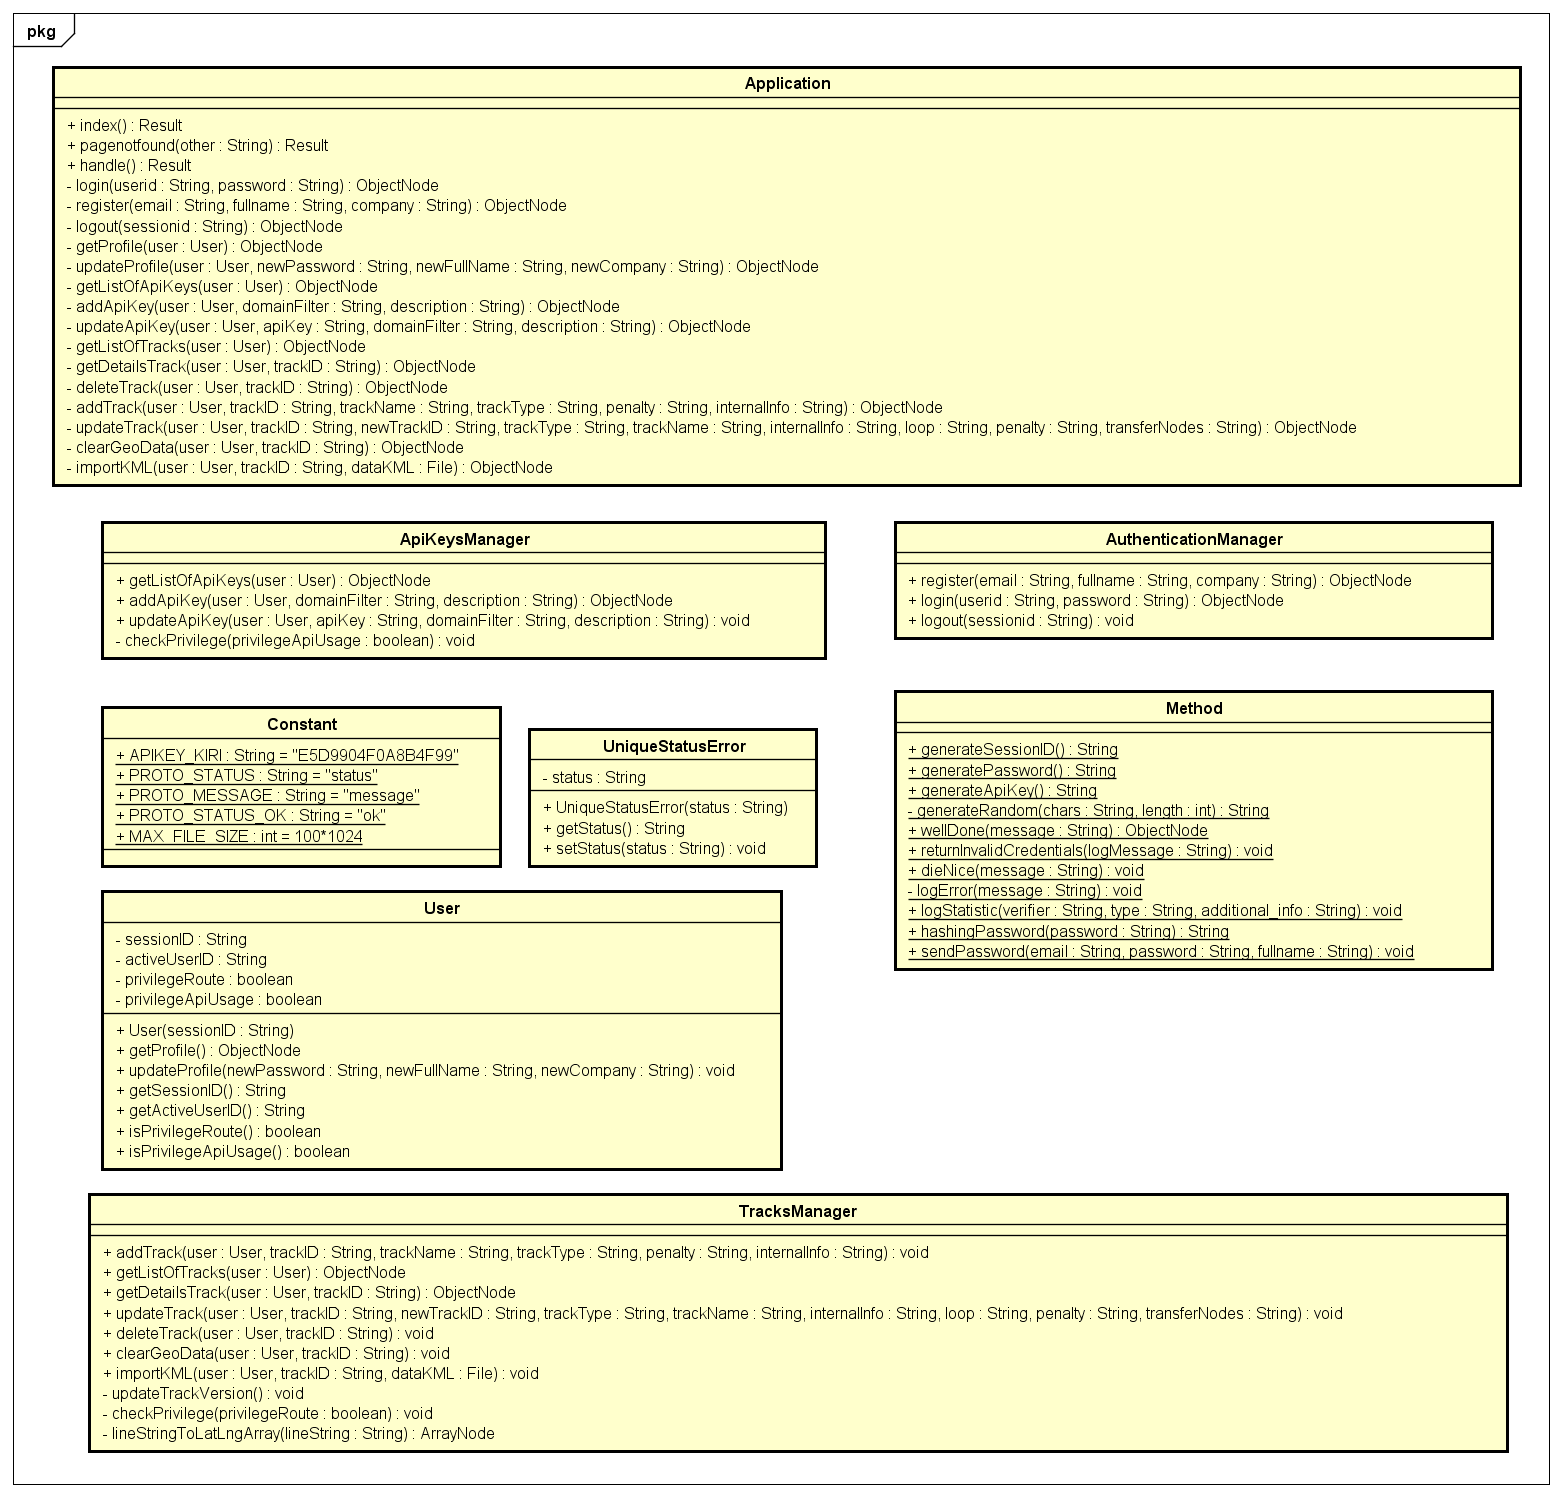
\includegraphics[scale=0.45]{Gambar/4_classdiagram.png}
	\caption{Kelas Diagram KIRI \textit{Dashboard Server Side}}
	\label{fig:4_classdiagram}
\end{figure}

\section{\textit{Controllers}}
\label{sec:controllerssrancangan}
\textit{Controllers} terdiri dari sebuah kelas, yaitu kelas Application. Kelas Application digunakan untuk menerima permintaan dari bagian tampilan sistem usulan dan digunakan juga sebagai pengirim pesan untuk membalas permintaan dari bagian tampilan. Deskripsi seluruh \textit{method} dari kelas Application adalah sebagai berikut:
\begin{itemize}
	\item \texttt{public Result index()}\\
	Berfungsi untuk mengarahkan pengguna ke halaman ``/bukitjarian/''.\\
	Nilai kembalian: halaman \textit{login} KIRI \textit{Dashboard}.
	\item \texttt{public Result pagenotfound(String other)}\\
	Berfungsi untuk memberikan informasi kepada pengguna bahwa halaman yang dituju tidak ada dalam sistem.\\
	Parameter:
	\begin{itemize}
		\item \texttt{other} halaman yang dituju.
	\end{itemize}
	Nilai kembalian: halaman \textit{page not found}.
	\item \texttt{public Result handle()}\\
	Berfungsi untuk menangani pembagian 16 permintaan pengguna (16 bagian yang telah dijelaskan pada bab analisis).\\
	Nilai kembalian: pesan berhasil/kesalahan dalam format JSON yang sesuai dengan permintaan pengguna.
	\item \texttt{private ObjectNode login(String userid, String password)}\\
	Berfungsi untuk menangani permintaan \textit{login}.\\
	Parameter:
	\begin{itemize}
		\item \texttt{userid} \textit{username} pengguna.
		\item \texttt{password} \textit{password} pengguna.
	\end{itemize}
	Nilai kembalian: pesan dalam format JSON yang berisi sesi id, hak akses terhadap rute, dan hak akses terhadap API \textit{keys}.
	\item \texttt{private ObjectNode register(String email, String fullname, String company)}\\
	Berfungsi untuk menangani permintaan \textit{register}.\\
	Parameter:
	\begin{itemize}
		\item \texttt{email} \textit{email} pengguna.
		\item \texttt{fullname} nama lengkap pengguna.
		\item \texttt{company} nama perusahaan pengguna.
	\end{itemize}
	Nilai kembalian: pesan dalam format JSON yang menandakan \textit{register} berhasil.
	\item \texttt{private ObjectNode logout(String sessionid)}\\
	Berfungsi untuk menangani permintaan \textit{logout}.\\
	Parameter:
	\begin{itemize}
		\item \texttt{sessionid} sesi id yang didapat ketika pengguna berhasil \textit{login}.
	\end{itemize}
	Nilai kembalian: pesan dalam format JSON yang menandakan \textit{logout} berhasil.
	\item \texttt{private ObjectNode getProfile(User user)}\\
	Berfungsi untuk menangani permintaan melihat data pribadi pengguna.\\
	Parameter:
	\begin{itemize}
		\item \texttt{user} data sesi dan hak akses yang dimiliki pengguna.
	\end{itemize}
	Nilai kembalian: pesan dalam format JSON yang berisi nama lengkap dan nama perusahaan pengguna.
	\item \texttt{private ObjectNode updateProfile(User user, String newPassword, String newFullName, String newCompany)}\\
	Berfungsi untuk mengubah data pribadi pengguna.\\
	Parameter:
	\begin{itemize}
		\item \texttt{user} data sesi dan hak akses yang dimiliki pengguna.
		\item \texttt{newPassword} \textit{password} baru pengguna.
		\item \texttt{newFullName} nama lengkap baru pengguna
		\item \texttt{newCompany} nama perusahaan baru pengguna
	\end{itemize}
	Nilai kembalian: pesan dalam format JSON yang menandakan bahwa mengubah data pribadi pengguna berhasil.
	\item \texttt{private ObjectNode getListOfApiKeys(User user)}\\
	Berfungsi untuk melihat daftar API \textit{keys} yang dimiliki pengguna.\\
	Parameter:
	\begin{itemize}
		\item \texttt{user} data sesi dan hak akses yang dimiliki pengguna.
	\end{itemize}
	Nilai kembalian: pesan dalam format JSON yang berisi daftar API \textit{keys} pengguna.
	\item \texttt{5 method lainnya}\\
\end{itemize}

\section{\textit{Models}}
\label{sec:modelsrancangan}
\textit{Models} terdiri dari 7 buah kelas. \textit{Models} merupakan bagian pada Play Framework yang melakukan pemroresan data secara detail. Deskripsi kelas beserta fungsi dari kelas tersebut akan dijelaskan ke dalam subbab selanjutnya.

\subsection{ApiKeysManager}
\label{sec:apikeysmanager}
Kelas ini merupakan kelas untuk mengelola data-data API \textit{keys} yang dimiliki oleh pengguna KIRI \textit{Dashboard}. Kelas ini untuk menangani permintaan: bagian melihat daftar API \textit{keys}, menambahkan API \textit{keys} dan mengubah API \textit{keys}. Berikut adalah seluruh \textit{method} yang digunakan pada kelas ini:
\begin{itemize}
	\item \texttt{public ObjectNode getListOfApiKeys(User user)}\\
	Berfungsi untuk mendapatkan daftar API \textit{keys} pengguna\\
	Parameter:
	\begin{itemize}
		\item \texttt{user} data sesi dan hak akses yang dimiliki pengguna.
	\end{itemize}
	Nilai kembalian: objek JSON yang berisi daftar API \textit{keys} pengguna.
	\item \texttt{public ObjectNode addApiKey(User user, String domainFilter, String description)}\\
	\item \texttt{public void updateApiKey(User user, String apiKey, String domainFilter, String description)}\\
	\item \texttt{private void checkPrivilege(boolean privilegeApiUsage)}\\
	\item \texttt{private String generateApiKey()}\\
\end{itemize}

\subsection{AuthenticationManager}
\label{sec:authenticationmanager}

\subsection{Constant}
\label{sec:constant}

\subsection{TracksManager}
\label{sec:tracksmanager}

\subsection{UniqueStatusError}
\label{sec:uniquestatuserror}

\subsection{User}
\label{sec:user}

\subsection{Utils}
\label{sec:utils}

\section{\textit{Views}}
\label{sec:viewssrancangan}
Disalin apa adanya.
